\chapter{Аналитическая часть}

В данном разделе представлено теоретическое описание КРМ-схемы хранения разреженных матриц и заданного алгоритма.

\section{КРМ-схема хранения разреженных матриц}

Для начала следует описать схему хранения разреженной матрицы, предложенную Кнутом. Ненулевые элементы хранятся в компактной форме в одномерном массиве $AN$. Информация о положении ненулевых элементов в матрице хранится двумя дополнительными параллельными одномерными массивами --- $I$ и $J$; здесь для каждого ненулевого элемента содержатся его строчный и столбцовый индексы. Итак, для каждого $a_{ij} \neq 0$ в памяти находится тройка $(a_{ij}, i, j)$. Далее, чтобы можно было легко отыскивать элементы произвольной строки или столбца матрицы, необходимы еще пара указателей для каждой тройки, а также указатели входа для строк и столбцов, сообщающие начало каждого строчного или столбцового списка. Пусть NR («next nonzero element in the same row» --- «следующий ненулевой элемент той же строки») --- массив, хранящий строчные указатели, а NC («next nonzero element in the same column» --- «следующий ненулевой элемент того же столбца») --- массив столбцовых указателей.
Пять массивов AN, I, J, NR и NC имеют одинаковую длину, и их одноименные позиции соответствуют друг другу. Пусть JR и JC --- массивы, содержащие указатели входа для строк и столбцов, расположенные в соответствии с порядком строк и столбцов матрицы. Тогда рассмотрим матрицу на рис. \ref{img:matrix}, её представление с помощью схемы Кнута --- на рис. \ref{img:knuth}.

\begin{figure}[H]
	\begin{center}
		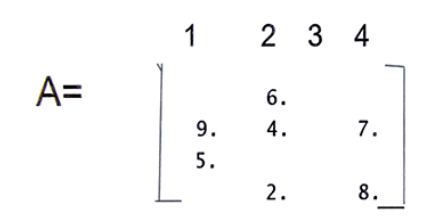
\includegraphics[scale=0.7]{img/matrix.png}
	\end{center}
	\captionsetup{justification=centering}
	\caption{Разреженная матрица}
	\label{img:matrix}
\end{figure}

\begin{figure}[H]
	\begin{center}
		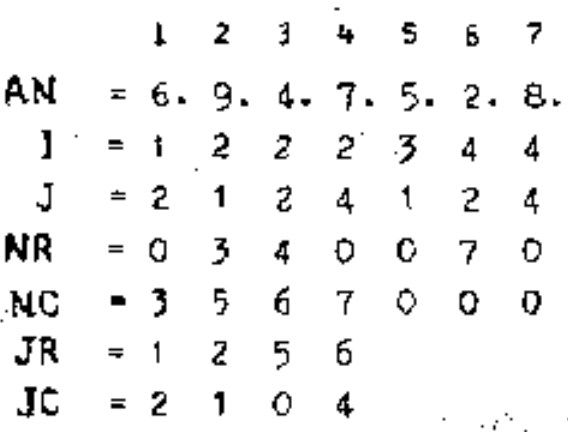
\includegraphics[scale=0.7]{img/knuth.png}
	\end{center}
	\captionsetup{justification=centering}
	\caption{Схема Кнута}
	\label{img:knuth}
\end{figure}

Рейнболдт и Местеньи предложили модификацию схемы Кнута, сохраняющую ее ценные свойства, но использующую значительно меньше накладных расходов по памяти. Она получила название схемы Кнута-Рейнбол-дта-Местеньи, или кольцевая КРМ-схема. Связные списки строк и столбцов закольцовываются, а начальные позиции списков включаются в указатели входа. Списки, ассоциированные со строками (столбцами), попарно не пересекаются и потому могут быть совместно хранимы одним массивом NR (для столбцов --- NC). Для матрицы на рис. \ref{img:matrix} \cite{tads} приведено ее представление с помощью КРМ-схемы на рис. \ref{img:krm}. Эта схема более плотная по сравнению со схемой Кнута. Однако, если приходится просматривать элементы некоторой строки (или столбца), то в сжатом формате нет никакой информации о столбцовых (строчных) индексах этих элементов~\cite{krm}.

\begin{figure}[H]
	\begin{center}
		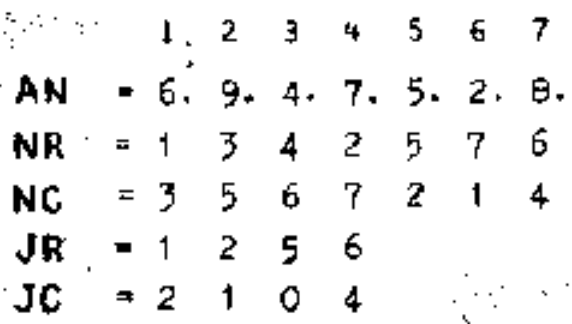
\includegraphics[scale=0.7]{img/krm.png}
	\end{center}
	\captionsetup{justification=centering}
	\caption{Кольцевая КРМ-схема}
	\label{img:krm}
\end{figure}

\section{Описание алгоритма}

Для получения из верхнетреугольной матрицы набора матриц, из которых исключены значения, меньшие $k$, где $k\in [1,Q]$ ($Q$ является входом алгоритма), необходимо в цикле по $k$, $k\in [1,Q]$, на каждой итерации удалить элементы, большие $k$. Для удаления элемента из матрицы нужно удалить его из массива $AN$, хранящего значения ненулевых элементов. Затем в массивах $NR$ и $NC$ изменить следующее: тот, кто ссылался на удаляемый элемент, теперь должен ссылаться на элемент, на который ссылался удаляемый. Значения номеров элементов, большие удаляемого, в массивах $NR$ и $NC$ должны уменьшиться на 1. В массивах $JR$ и $JC$ в случае, когда удаляется последний элемент в строке (столбце) записать 0 в позицию массива $JR$ ($JC$), равную номеру строки. В остальных случаях, когда удаляемый элемент является первым в строке (столбце) и в этой строке (столбце) есть другие элементы, надо вместо номера удаляемого элемента в массив $JR$ ($JC$) записать номер элемента, на который ссылается удаляемый элемент в массиве $NR$ ($NC$). Значения номеров элементов, большие удаляемого, в массивах $JR$ и $JC$ также должны уменьшиться на 1.

\section*{Вывод}

В данном разделе были описаны основные положения КРМ-схемы хранения разреженных матриц и заданного вариантом алгоритма обработки упакованной разреженной матрицы.